\documentclass[a4paper]{article}
\usepackage[utf8]{inputenc}
\usepackage{amsmath}
\usepackage{amssymb}
\usepackage{caption}
\usepackage{mathtools}
\usepackage{amsfonts}
\usepackage{lastpage}
\usepackage{tikz}
\usepackage{float}
\usepackage{textcomp}
\usetikzlibrary{patterns}
\usepackage{pdfpages}
\usepackage{gauss}
\usepackage{fancyvrb}
\usepackage[table]{colortbl}
\usepackage{fancyhdr}
\usepackage{graphicx}
\usepackage[margin=2.5 cm]{geometry}

\definecolor{listinggray}{gray}{0.9}
\usepackage{listings}
\lstset{
	language=,
	literate=
		{æ}{{\ae}}1
		{ø}{{\o}}1
		{å}{{\aa}}1
		{Æ}{{\AE}}1
		{Ø}{{\O}}1
		{Å}{{\AA}}1,
	backgroundcolor=\color{listinggray},
	tabsize=3,
	rulecolor=,
	basicstyle=\scriptsize,
	upquote=true,
	aboveskip={0.2\baselineskip},
	columns=fixed,
	showstringspaces=false,
	extendedchars=true,
	breaklines=true,
	prebreak =\raisebox{0ex}[0ex][0ex]{\ensuremath{\hookleftarrow}},
	frame=single,
	showtabs=false,
	showspaces=false,
	showlines=true,
	showstringspaces=false,
	identifierstyle=\ttfamily,
	keywordstyle=\color[rgb]{0,0,1},
	commentstyle=\color[rgb]{0.133,0.545,0.133},
	stringstyle=\color[rgb]{0.627,0.126,0.941},
  moredelim=**[is][\color{blue}]{@}{@},
}

\lstdefinestyle{base}{
  emptylines=1,
  breaklines=true,
  basicstyle=\ttfamily\color{black},
}

\pagestyle{fancy}
\def\checkmark{\tikz\fill[scale=0.4](0,.35) -- (.25,0) -- (1,.7) -- (.25,.15) -- cycle;}
\newcommand*\circled[1]{\tikz[baseline=(char.base)]{
            \node[shape=circle,draw,inner sep=2pt] (char) {#1};}}
\newcommand*\squared[1]{%
  \tikz[baseline=(R.base)]\node[draw,rectangle,inner sep=0.5pt](R) {#1};\!}
\newcommand{\comment}[1]{%
  \text{\phantom{(#1)}} \tag{#1}}
\def\el{[\![}
\def\er{]\!]}
\def\dpip{|\!|}
\def\MeanN{\frac{1}{N}\sum^N_{n=1}}
\cfoot{Page \thepage\ of \pageref{LastPage}}
\DeclareGraphicsExtensions{.pdf,.png,.jpg}
\author{Nikolaj Dybdahl Rathcke (rfq695)}
\title{Graph Coloring \\ Assignment 1}
\lhead{Graph Coloring}
\rhead{Assignment 1}

\begin{document}
\maketitle

\section{Problem 1}
The first step of a \texttt{FunnyGraph}, $F(n)$, is to remove a cycle from a complete graph $G$. Say the graph has $n$ vertices, so the starting graph has $\chi(G)=n$. Removing the cycle results in the graph $G'$ with $\chi(G')=\lceil \frac{n}{2} \rceil$. To see this is correct, consider the coloring where two vertices that were adjacent in the removed cycle are colored with the same color. Thus, if $n$ is even, then it can be done with $n/2$ colors, and if $n$ is odd, then we have a vertex left over, so we must use $\lceil \frac{n}{2} \rceil$ colors. To prove this is an optimal coloring, we use the formula
\begin{align*}
  \frac{|V(G)|}{\alpha (G)}\leq \chi(G)
\end{align*}
Since the maximum independent set can easily be seen to be $2$, that means it is optimal to color sets of $2$ as the left hand side is exactly equal to $\chi(G')$ when $n$ is even. It is also optimal when $n$ is odd as we can not have an independent set of $3$. \\
The second step is the Mycielskistep, which increases the chromatic number of a graph by $1$. So now we have a graph $G''$ with $\chi(G'')=\lceil \frac{n}{2} \rceil+1$. \\
The last step is to join it with the wheel graph $W_{n+1}$. The wheel graph has chromatic number $3$ when $n+1$ is odd, and chromatic number $4$ when $n+1$ is even. Since joining two graphs makes the graphs completely connected, they cannot have any of the same colors. Now we know that
\begin{align*}
  \chi(G_1+\cdots +G_n)=\sum_{i=1}^n \chi(G_i)
\end{align*}
So the resulting graph, $G'''$, has chromatic number $\chi(G''')=\chi(G'')+\chi(W_{n+1})$, so the chromatic number of the \texttt{FunnyGraph} of size $n$ can be expressed as:
\begin{align*}
  \chi(F(n)) =
  \begin{cases} \lceil \frac{n}{2} \rceil + 5 & \text{if $n$ is odd} \\
                \frac{n}{2} + 4               & \text{if $n$ is even}
  \end{cases}
\end{align*}
As $W_{n+1}$ will have an odd cycle when $n$ is odd and the other way around. We can also remove the ceilings as we know $n/2$ will give us an integer for even $n$. So for $G=F(99)$, the chromatic number is $\lceil \frac{n}{2} \rceil + 5=55$. Note that the expression for $\chi(F(n))$ only works for $n\geq 4$.

\section{Problem 2}
To prove that this greedy method does not provide optimal results, I will show a counter example which can be extended to make infinitely many graphs where it is not optimal. Consider the following graph $G$:
\begin{figure}[H]
  \centering
  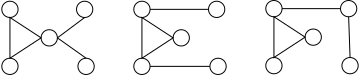
\includegraphics[scale=0.75]{fig1.pdf}
\end{figure}
It is constructed by $K_3$ in the middle, and then adding three new vertices, which connect to two of the vertices from $K_3$. The proposed greedy method would pick the three outer vertices as it is the largest independent set. Then only $K_3$ would be left, which requires $3$ colors, so the coloring would use a total of $4$ colors. However, it is optimal to pick independent sets of size $2$, the sets that pick one vertex for the inner and outer "triangle". This results in a coloring using only $3$ colors. \\
This can be extended by adding infinity many of these "triangles" on the outside that connects to $K_3$ in the same way. The largest independent set will always have size $|V(G)|-3$, where the last $3$ vertices are in $K_3$, so the greedy method will always use $4$ colors, while it is optimal to pick $3$ equally large sets, one vertex from each "triangle", as it uses only $3$ colors. This can actually be extended for any $K_n$ as long as you add $n$ vertices that connects to $n-1$ vertices from $K_n$ for each "iteration" of this.

\section{Problem 3}
Say we have an optimal coloring of $G$ using $\chi(G)$ colors. Then we have a partition of $G$ into $n$ ($=\chi(G)$) independent sets. Let these sets have size $\alpha_1(G),..,\alpha_n(G)$. We know that at least one of the independent sets has size larger than or equal to $\frac{|V(G)|}{\chi(G)}$, since otherwise all vertices are not colored. Therefore we can say that:
\begin{align*}
  \frac{|V(G)|}{\chi(G)}&\leq \max(\alpha_i(G)) \comment{For $i=1..n$} \\
                        &=\max(\omega_i(\overline{G})) \comment{As $\omega(\overline{G})=\alpha(G)$} \\
                        &\leq \chi(\overline{G}) \comment{Since $\omega(\overline{G})\leq \chi({G})$}
\end{align*}
If we now multiply both sides by $\chi(G)$, we get:
\begin{align*}
  |V(G)|&\leq \chi(\overline{G})\chi(G)
\end{align*}
We now easily see that either $\chi(\overline{G})$ or $\chi(G)$ must be larger than or equal to $\sqrt{|V(G)|}$, as the above inequality would not hold otherwise, therefore we have:
\begin{align*}
  \max(\chi(G), \chi(\overline{G}))\geq \sqrt{|V(G)|}
\end{align*}
Which is what we wanted to show.

\section{Problem 4}
We start by proving that $\omega(G)\chi(H)\leq \chi(G[H])$. We know that for any graph $G'$, then $\omega(G')\leq \chi(G')$. Since the graph $H$ has chromatic number $\chi(H)$, the substituted graph $G[H]$ must use $\omega(G)\cdot \chi(H)$ colors as the clique consisting of $\omega(G)$ components of $H$ is completely connected, since when they are completely connected, it means that any two components cannot use the same color. Thus, it holds that $\omega(G)\chi(H)\leq \chi(G[H])$. \\
\\
Now we need to prove that $\chi(G[H])\leq \chi(G)\chi(H)$. Let us denote $V_i$ the vertex $i$ in $G$ and let $H_i$ be the graph $H$ replacing the vertex $V_i$. Let their (optimal) colorings be denoted $c(V_i)$ and $c(H_i)$ (remember that each $H_i$ can be colored differently). If we had an optimal coloring of $G$, then using the same coloring where each component in $G[H]$ has optimal coloring $c(H_i)$ whenever $G$ had coloring $c(V_i)$ must produce a coloring of $G[H]$ using at most $\chi(G)\chi(H)$ colors. Note that it is only an upper bound since colorings of $H_i$ and $H_j$ might use \textit{some} of the same colors when they are not adjacent, but can still be different colorings even though both uses $\chi(H)$ colors. If we use entirely different set of colors (as we are forced to do if the components are adjacent) for all components $H_i$ having a different coloring, then we have exactly that $\chi(G[H])=\chi(G)\chi(H)$. \\
\\
To demonstrate that it is in fact an upper bound and not an exact bound, consider $G[H]$, where $G=C_5$ and $H=K_2$. Since each component after the substitution is completely connected if there was an edge in $G$, we cannot use any of the same colors for two adjacent components. Each component $H_i$ in the substituted graph requires $2$ colors. We can perform the following coloring of $G[H]$:
\begin{figure}[H]
  \centering
  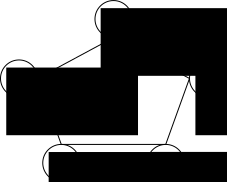
\includegraphics[scale=0.9]{fig2.pdf}
\end{figure}
Since $\chi(G)=3$ as it is an odd cycle and $\chi(H)=2$, the upper bound is $6$. However, this coloring only uses $5$ colors, which means it is possible to have $\chi(G[H])<\chi(G)\chi(H)$.

\section{Problem 5}
The chromatic number of the constructed graph $G$ of size $n$ as described in the assignment text is equal to $\pi(n)$, where $\pi$ is the function that counts primes under $n$ plus one. The plus one comes from the number $1$. Thus the chromatic number, $\chi(G)$, for $n=20162016$ is $\pi(20162016)=1280233$. \\
\\
\texttt{Proof:} Imagine we introduce vertex $1$ first and iteratively adds vertices in order so that the last vertex that is introduced is $V_n$. The proof consists of two parts. Firstly, we want to prove that every time we introduce a prime-numbered vertex, we need an additional color. And secondly, when we introduce a composite-numbered vertex, we do not need any additional colors.\\
The first part is easy to see. Say we introduce a prime-numbered vertex $V_p$. Then for any prime $q$, where $q<p$, then $\gcd(q,p)=1$ or $p$ would not be a prime. This means there is an edge to all primes less than $p$. Thus all primes (and including $1$) must form a clique in $G$. \\
For the second part, when we introduce a composite-numbered vertex $V_k$, then $k$ has a prime factorization. We know that $k$ is divisible by any of these prime factors, thus there cannot be an edge between two of these vertices. So if we color $V_k$ the same as any of the prime factors, we have a valid coloring of $G$. To see this is true, we prove it by contradiction. Suppose we have a vertex $V_l$ where there is an edge to $V_k$, so $\gcd(l,k)=1$. If the vertices were colored the same, then it means that $l$ and $k$ have a common prime factor $p$. But if this is true, then $p\mathop \backslash l$ and $p\mathop \backslash k$, which implies $\gcd(l,k)\neq 1$ as $p>1$. This is a contradiction, so this coloring must be a valid coloring of $G$. $\hfill\blacksquare$

\end{document}
